\chapter{Device Management Server}
\label{sec:devmgmtsrv}
%TODO : Review > Fokus Satz umschreiben
In diesem Kapitel wird der Device Management Server behandelt. Der Fokus liegt dabei auf der Spezifikation und deren technischen Umsetzung. Zielperson dieses Kapitels sind Entwickler sowie Personen, die an technischen Details Interesse haben.

\section{Software Analyse}

\subsection{Spezifikationen}
Um die Anforderungen zu evaluieren wurde das bestehende Geräteverwaltungsportal analysiert. Da beim bestehenden System der Funktionsumfang stark eingeschränkt war, wurde vom Industriepartner zusätzliche Funktionalität gewünscht.
Um eine kurze Übersicht über die vorhandenen Funktionen und erfassten Anforderungen zu geben folgt die Tabelle \ref{tab:anforderungendevmgmtsrv}.

\begin{longtable}{  p{3.5cm} | p{4.3cm} | p{4.3cm} }

    \textbf{Spezifikation} & \textbf{Altes System} & \textbf{Neues System} \\ [1ex] \hline \hline & &  \\ [-1.5ex]
    Einstellungen anpassen & Nur Renndistanzkorrektur & Detaillierte Verwaltung der Geräteeinstellungen\\ [1ex] \hline & &  \\ [-1.5ex]
    Status der Geräte & Rudimentäre Anzeige des Gerätestatus & Detaillierte Anzeige des Gerätestatus\\ [1ex] \hline & &  \\ [-1.5ex]
     Alarming bei schlechtem Gerätezustand & Dauer seit letztem Positionsupdate / Bildempfang zu gross & Visuelle Hervorhebung bei Problemen mit dem Gerätestatus \\ [1ex] \hline & &  \\ [-1.5ex]
    Neustarten des Gerätes & Neustarten des Gerätes via Portal & nur Neustarten der App möglich\\ [1ex] \hline & &  \\ [-1.5ex]
    Gerätelog anzeigen & - & Gerätelog anzeigen\\ [1ex] \hline & &  \\ [-1.5ex]
    Versand von Nachrichten & - & Versand von Nachrichten möglich\\ [1ex] 
\caption{Anforderungen Device Management Server}
\end{longtable}
\label{tab:anforderungendevmgmtsrv}

Eine detaillierte Beschreibung aller Anforderungen befindet sich im Anhang im Kapitel \ref{sec:anforderungenandroiddevmgmt}. Nachfolgend ein kurzer Überblick der wichtigsten Anforderungen.

\subsection{Funktionale Anforderungen}
\subsubsection{Betriebsmodi}
Die Geräte sollen sowohl über einen Management Server, analog zur bisherigen Verwaltungsseite, fernverwaltet als auch über ein „Einstellungen“-Menü direkt am Gerät konfiguriert werden können. 

Daraus resultieren zwei Betriebsmodi: «managed» (TourLive App wird über den Device Management Server verwaltet) und «unmanaged» (TourLive App wird in den lokalen App Einstellungen verwaltet). Die Standardkonfiguration sieht den Modus «managed» vor. Die beiden Modi lassen sich am Gerät wie auch auf dem Device Management Server jederzeit ändern. 


\subsubsection{Alarming Funktionen}
Treten Probleme auf, so soll auf dem Telefon sowie in der Management Konsole darüber informiert werden. Als zu meldende Probleme gelten folgende:
\begin{itemize}
\item Smartphone Akkustand liegt unter 30\%
\item Smartphone wird nicht mehr geladen (Stromzufuhr unterbrochen)
\item Keine Medien-Daten seit mehr als 3 Minuten
\item Keine Positions-Daten seit mehr als 3 Minuten
\item Keine Status Updates seit mehr als 3 Minuten
\item Weniger als 30\% freier Speicher intern und extern
\item Keine GPS-Satelliten verfügbar sind
\end{itemize}
	
\subsection{Technologien}
Für die Entwicklung des Device Management Servers wurden die selben Technologien verwendet, die bereits für den TourLive Server evaluiert wurden. Mehr Informationen dazu im Kapitel \ref{sec:tourliveserverevaluationwebframework} und \ref{sec:tourlivetechnologien}.

\subsection{Domain Model}
Abbildung \ref{fig:domainmodeldevmgmtsrv} zeigt das Domain Model des Device Management Servers. Das Domain Model kann grundsätzlich in vier Kategorien unterteilt werden. Jede dieser vier Kategorien wird jeweils einem Gerät (der Klasse \textit{Device.java}) assoziiert. Die vier Kategorien sind: 


\begin{itemize}
\item Die Klasse \textit{TourLiveLog.java} (1) mit sämtlichen Gerätelogs in Form der Klasse LogEntry. 
\item Die Klasse \textit{DeviceManagementContainer.java} (2), die die Geräteeinstellungen auf die Klassen \textit{DeviceSettings.java}, \textit{RecordingSettings.java} und \textit{AdditionalSettings.java}, aufteilt.
\item Die Klasse \textit{StatusData.java} (3), die den aktuellen Gesundheitszustand eines Aufnahmegerätes widerspiegelt.
\item Die Klasse \textit{Message.java} (4), die allfällige Nachrichten vom Device Management Server an ein Aufnahmegerät speichert.
\end{itemize}

\begin{figure}[H]
	\centering
	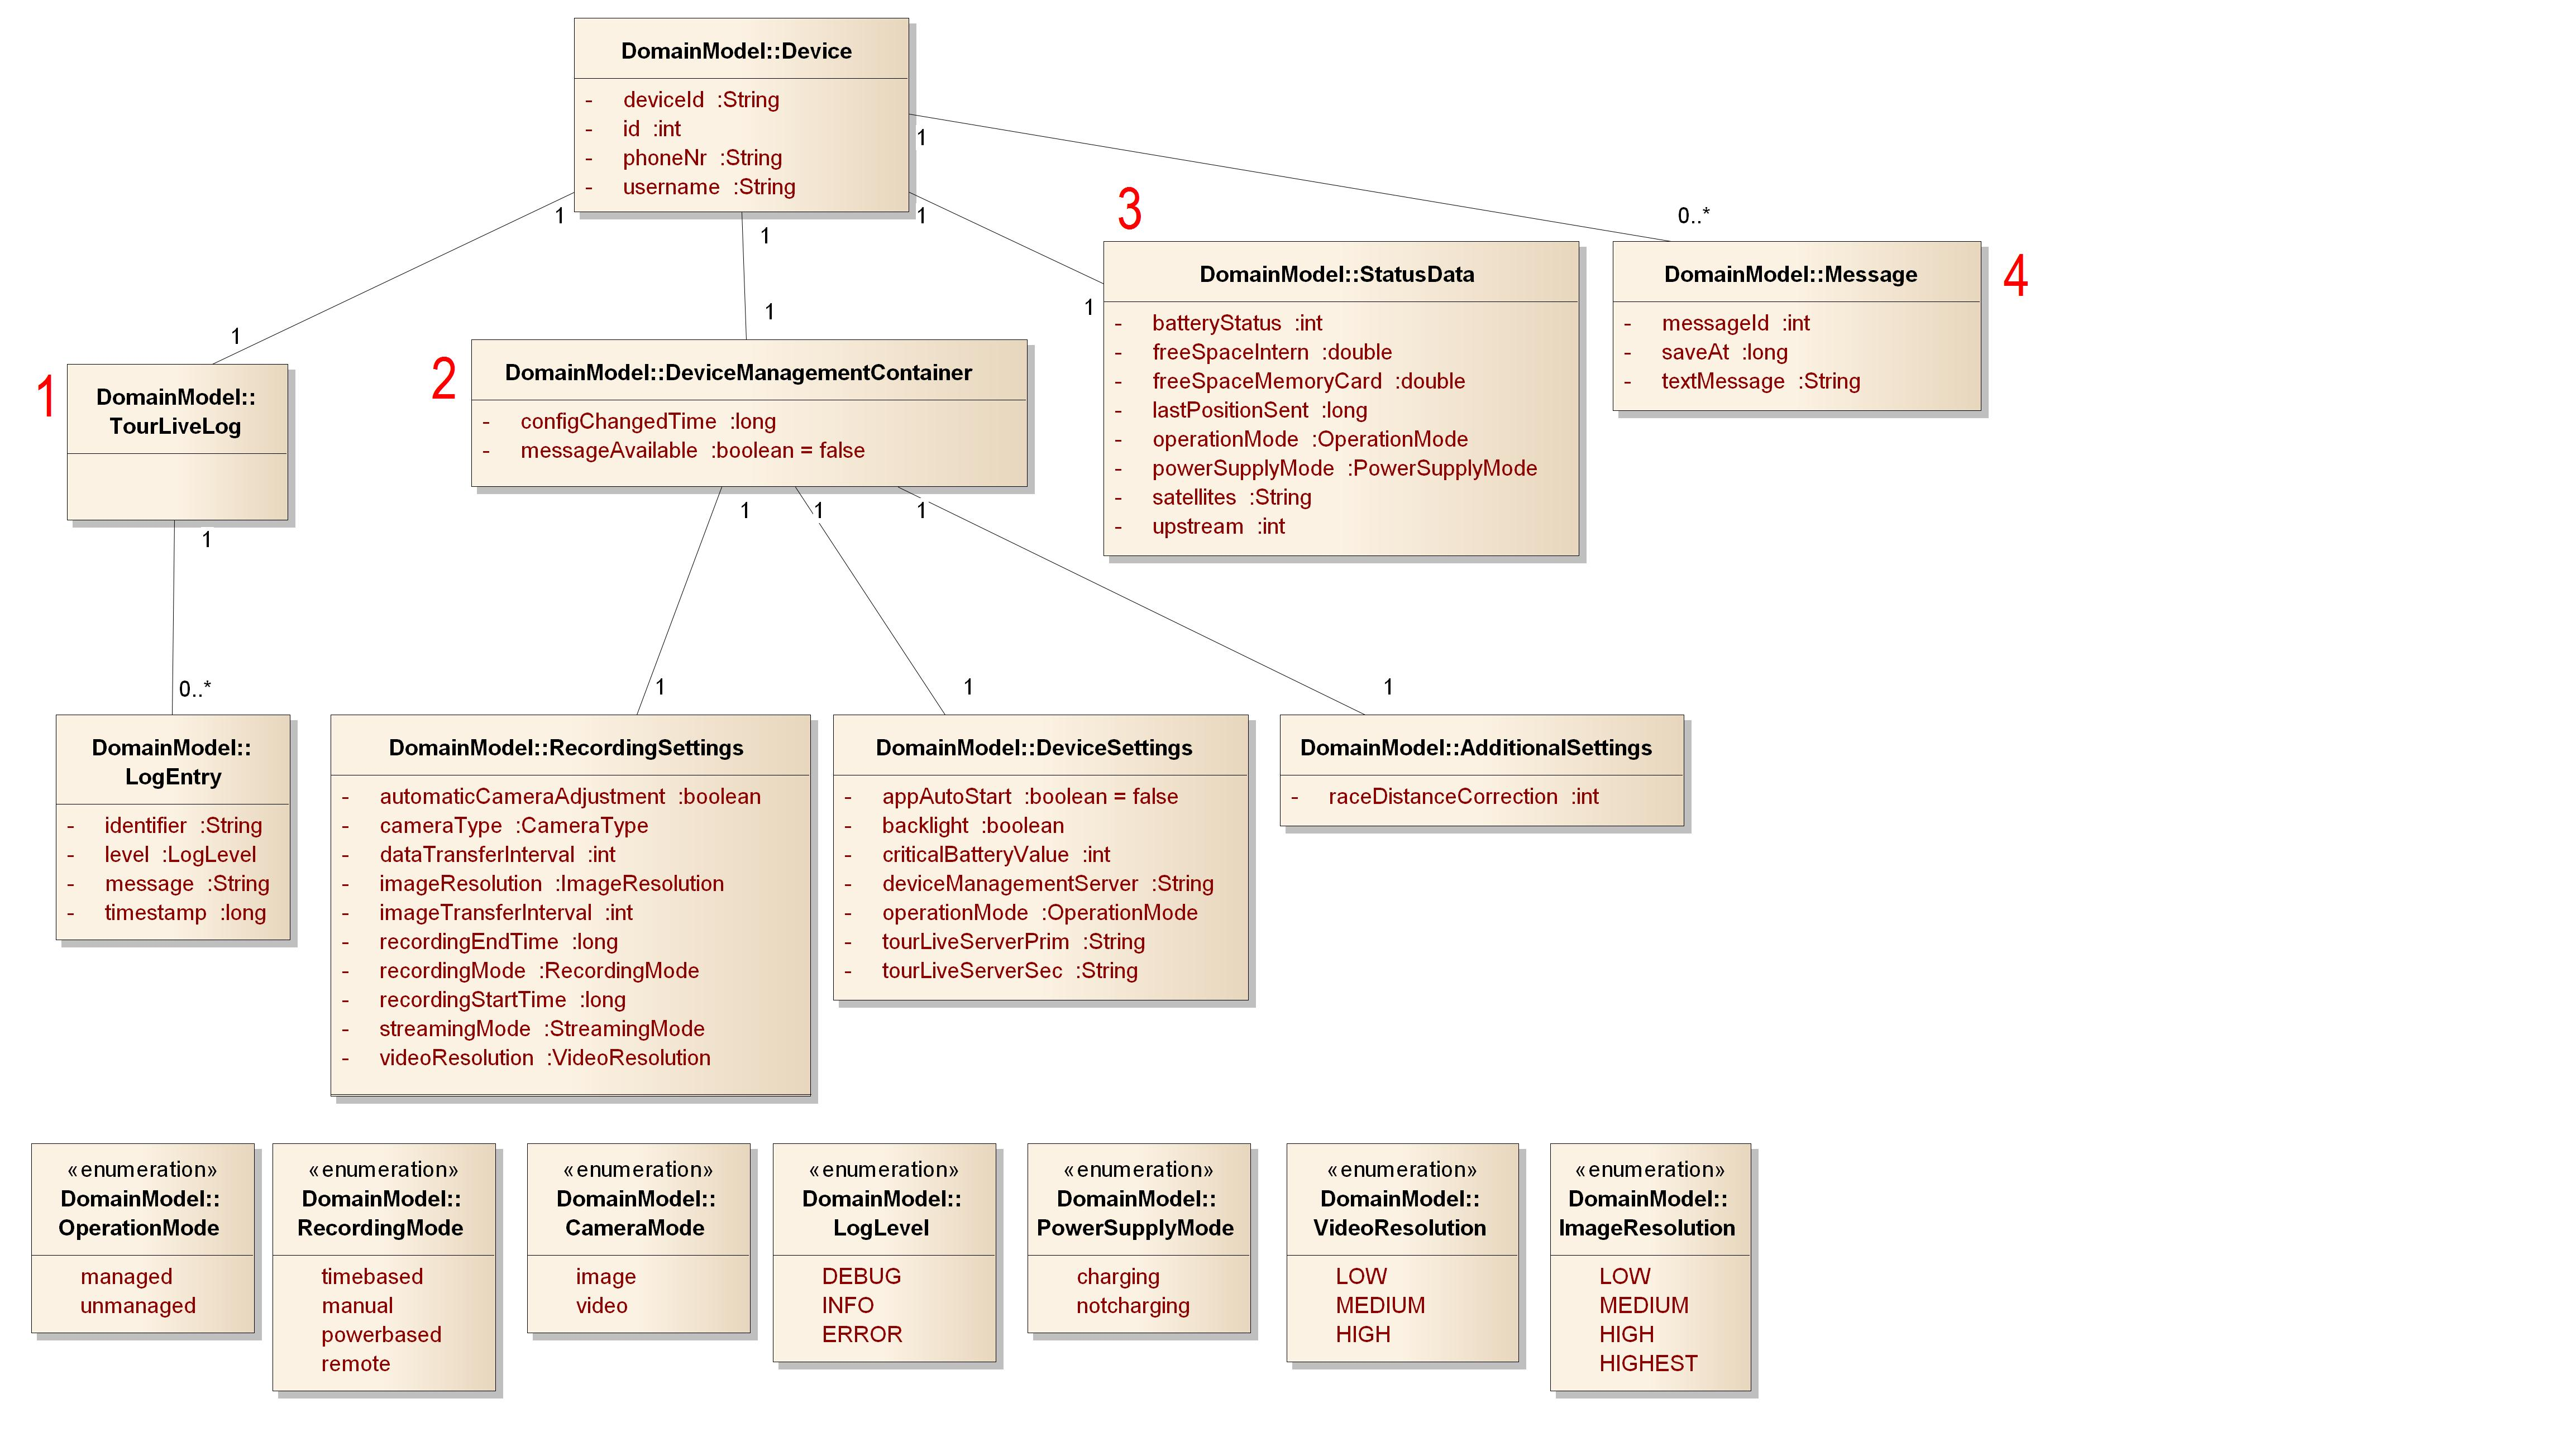
\includegraphics[width=130mm]{images/devmgmtsrv/domainmodel.jpg}
	\label{fig:domainmodeldevmgmtsrv}
	\caption{Domain Model des Device Management Servers}
\end{figure}


\section{Software Design}
\subsection{Architektur und Übersicht}
Der Device Management Server unterteilt sich in Webseite und API. Die API wird von den Aufnahmesystemen angesprochen wohingegen die Webseite hauptsächlich von Administratoren genutzt wird.



\begin{figure}[H]
	\centering
	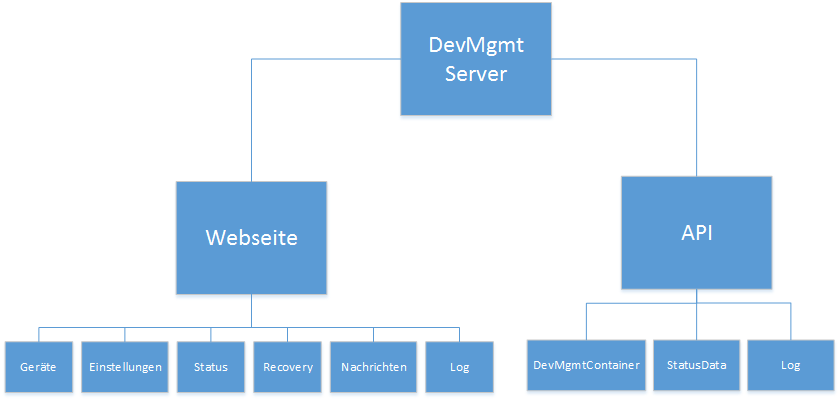
\includegraphics[width=130mm]{images/devmgmtsrv/uebersicht.png}
	\caption{Grobstruktur des Device Management Servers}
\end{figure}

Wie beim TourLive Server besteht dank der gewählten Struktur die Möglichkeit, die Webseite und die API auf verschiedene Server aufzuteilen. Da die Auslastung des Device Management Servers gering sein wird, wird darauf verzichtet.

\subsection{Schichtenmodell und Paketdiagramm}
Der Device Management Server ist in vier Schichten unterteilt. Die Schichten wurden an die vorgegebene Struktur des Spring Frameworks angepasst. Abbildung \ref{fig:devmgmtsrvschichten} zeigt diese vier Schichten auf. Jede Schicht kann nur auf die darunterliegenden Schichten zugreifen.

\begin{figure}[H]
	\centering
	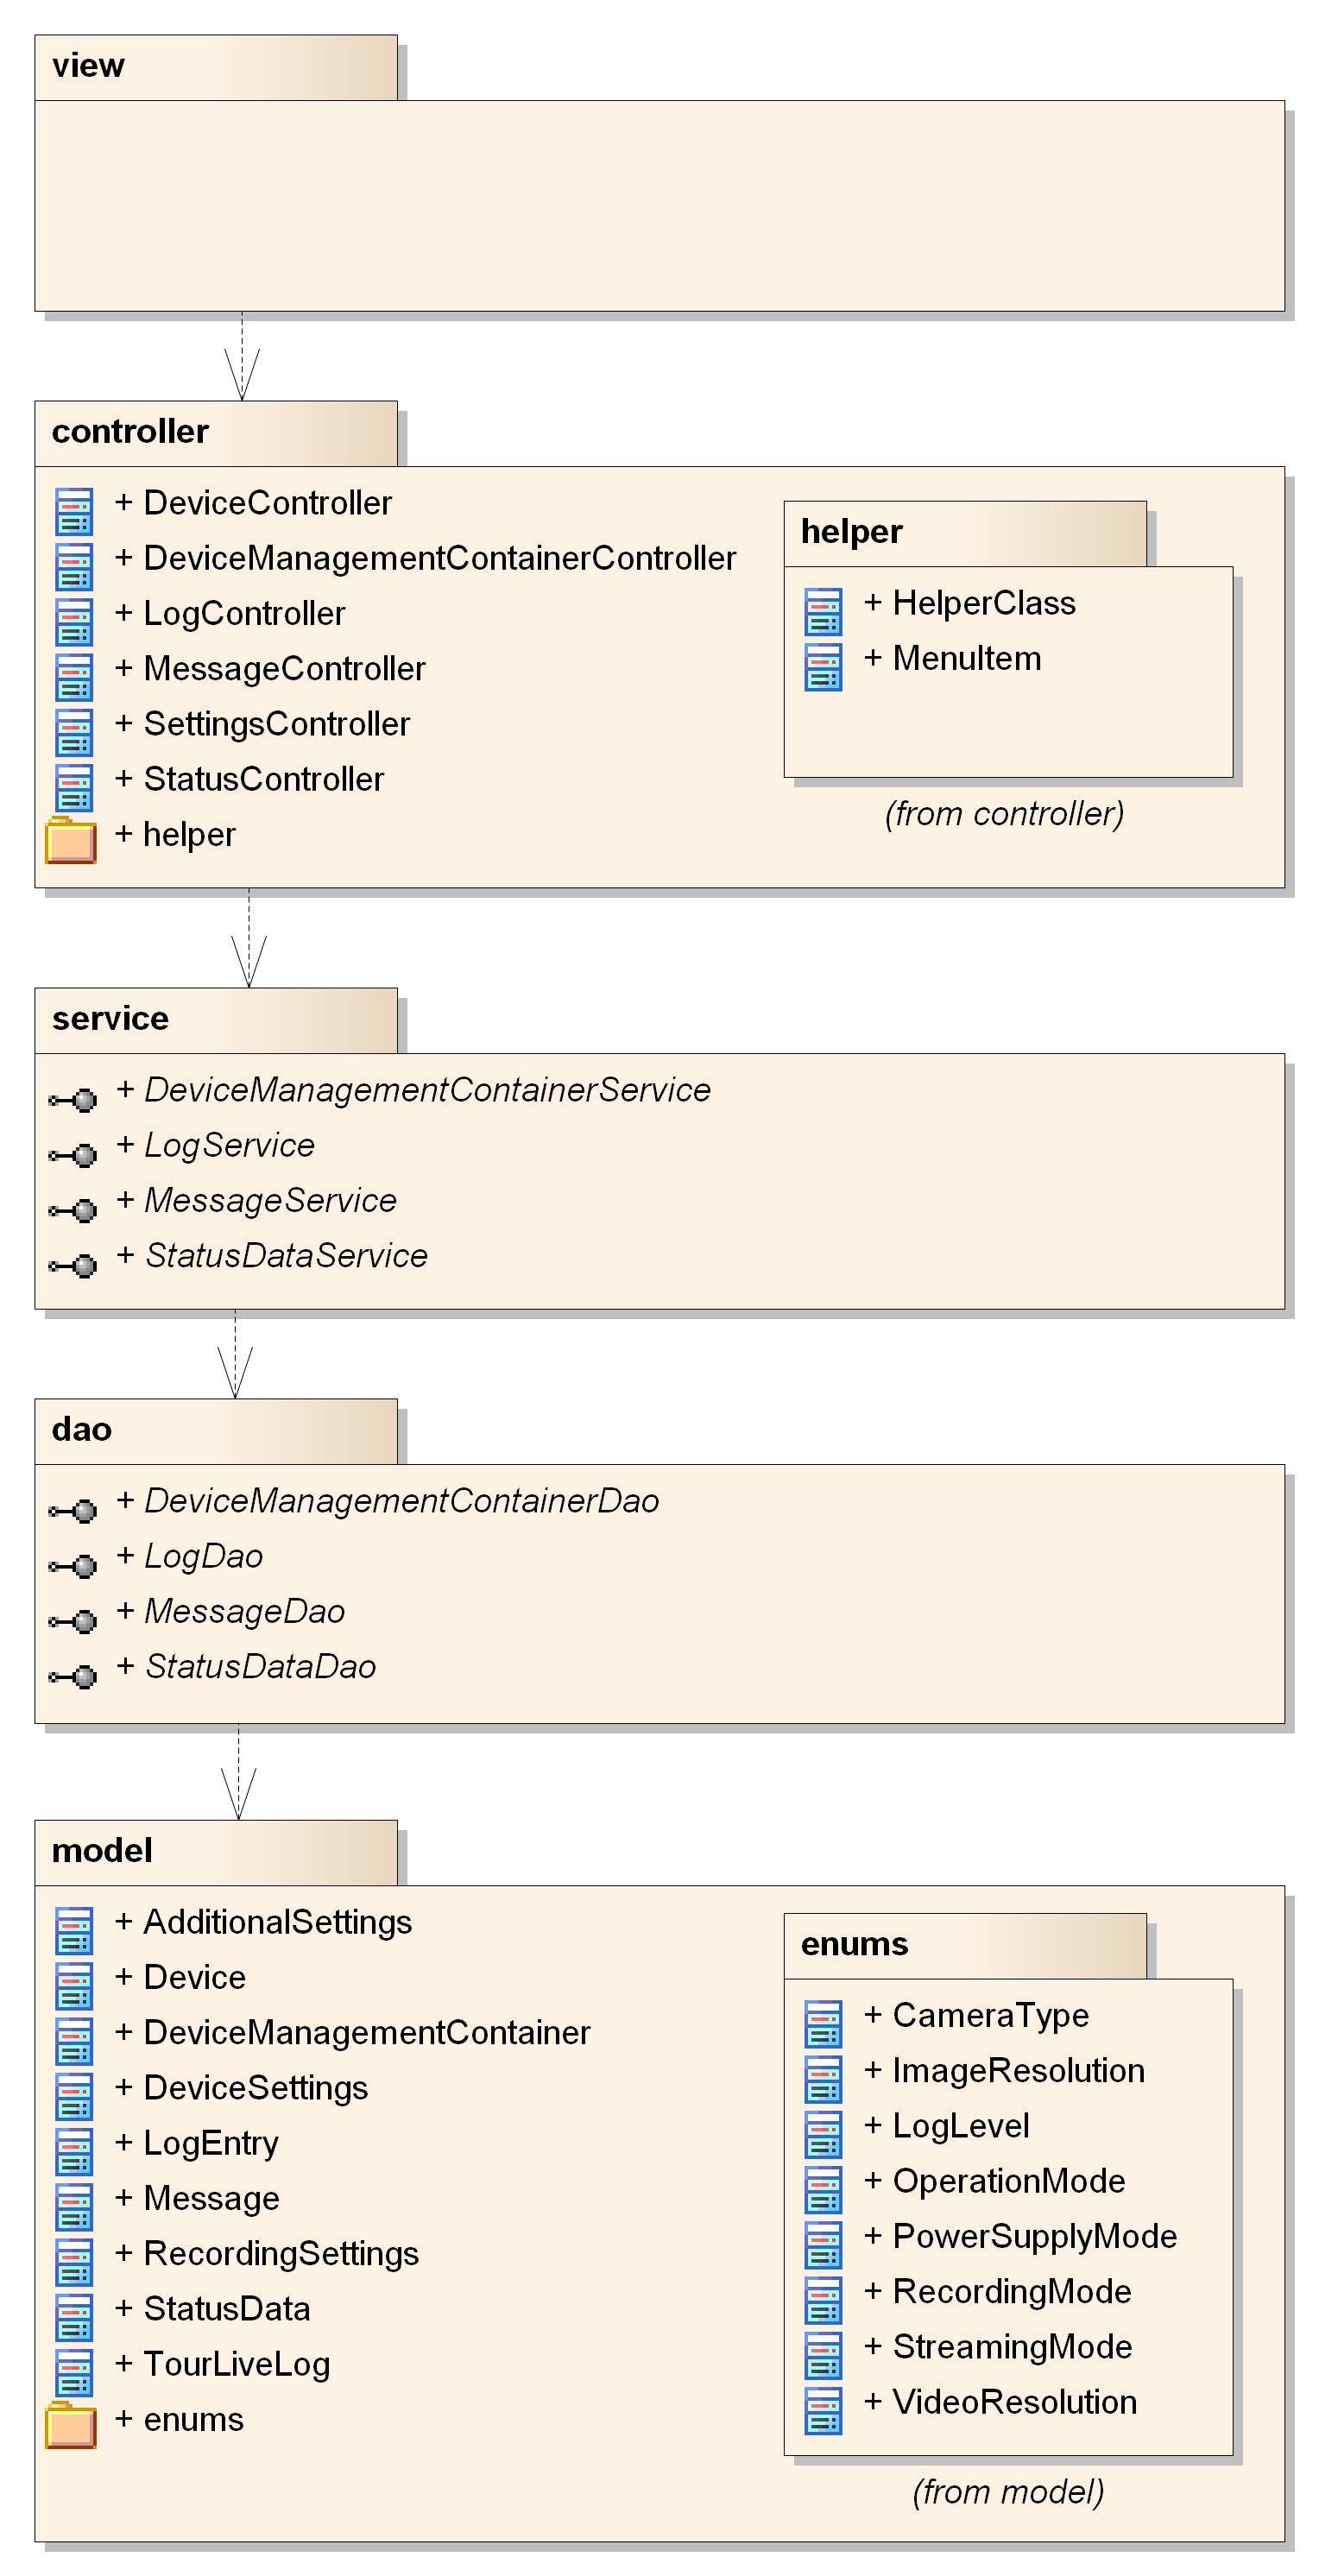
\includegraphics[width=80mm]{images/devmgmtsrv/schichten.jpg}
	\label{fig:devmgmtsrvschichten}
	\caption{Schichtendiagramm des Device Management Servers}
\end{figure}

\subsubsection{View}
Die View Schicht enthält alle *.jsp Dateien, die für die Darstellung der Webseite benötigt werden. 

\subsubsection{Controller}
Die Controller widerspiegeln die HTTP-Methoden (GET, POST,...) die für die Anzeige der Webseite und die RESTful JSON-Schnittstelle benötigt werden. Die Controller besitzen zwei verschiedene Methodentypen. Die einen werden für die Webseite zur Verfügung gestellt und die anderen für die Aufnahmesysteme. An den Methoden sieht man lediglich den Unterschied, dass bei den Webseitenemthoden ein ViewModel vorhanden ist, welches für die Anzeige gebraucht wird.

\subsubsection{Service}
Die Service Klassen sind für die Businesslogik auf den von den DAO's gelieferten Objekten verantwortlich.

\paragraph{Device Management Container Service}
Der Device Management Container Service speichert und liefert die Container mit den Geräteeinstellungen sowie das Flag \textit{'messageAvailable'} falls auf dem Device Management Portal eine Nachricht für das Gerät vorhanden ist.

\subsubsection{DAO}
Die DAO Schicht enthält die Datenzugriffsobjekte. Diese dient zur Entkopplung der Geschäftslogik vom Datenzugriff. Die Interfaces bilden die Schnittstelle, die Implementierung kann so je nach Persistenztechnologie unterschiedlich sein, ohne dass die Geschäftslogik geändert werden muss.


\subsubsection{Model}
Die Domäne des Device Management Servers wird in der Model Schicht abgebildet. In den Objektinstanzen der Model Klassen sind die eigentlichen Daten gespeichert. Diese Objektinstanzen werden über den OR-Mapper in der SQL-Datenbank gespeichert.



\section{Realisierung}
Folgendes Kapitel beschreibt die Umsetzung des Device Management Servers.

\subsection{Definition Requests}
Die Requests werden mittels Spring Annotations definiert. 

\begin{lstlisting}[language=Java, caption=Spring Annotation]
@RequestMapping(value = "/api/getdevmgmtcontainer", method = RequestMethod.POST)
@ResponseBody
public DeviceManagementContainer getDeviceManagementContainer(@RequestBody final StatusData request)

\end{lstlisting}

\begin{itemize}
\item \textbf{\textit{@RequestMapping}:} gibt an, welche URL auf diese Methode gemappt wird und welche HTTP Request Methode erlaubt ist.
\item\textbf{\textit{@ResponseBody}: } definiert, dass die Methode einen HTTP Response Body zurück gibt und nicht eine JSP-Seite rendert.
\item\textbf{\textit{@RequestBody}: } der Parameter der Methode wird als Body des Requests definiert.
\end{itemize}
Diese annotierten Methoden müssen in einer Klasse enthalten sein, welche als \textit{\textbf{@Controller}} annotiert ist.


\subsection{Webseite}
Die Webseiten wurden mit JSP umgesetzt und mit der JavaScript Library JQuery angereichert. Um die grafische Oberfläche möglichst einfach zu gestalten, wurde  Twitter Bootstrap \footnote{Twitter Bootstrap, \url{http://twitter.github.io/bootstrap/}, besucht am 25. Mai 2013} benutzt.

Die Webseite wird in drei Teile unterteilt, Header, Footer sowie den Hauptbereich. 

\begin{figure}[H]
	\centering
	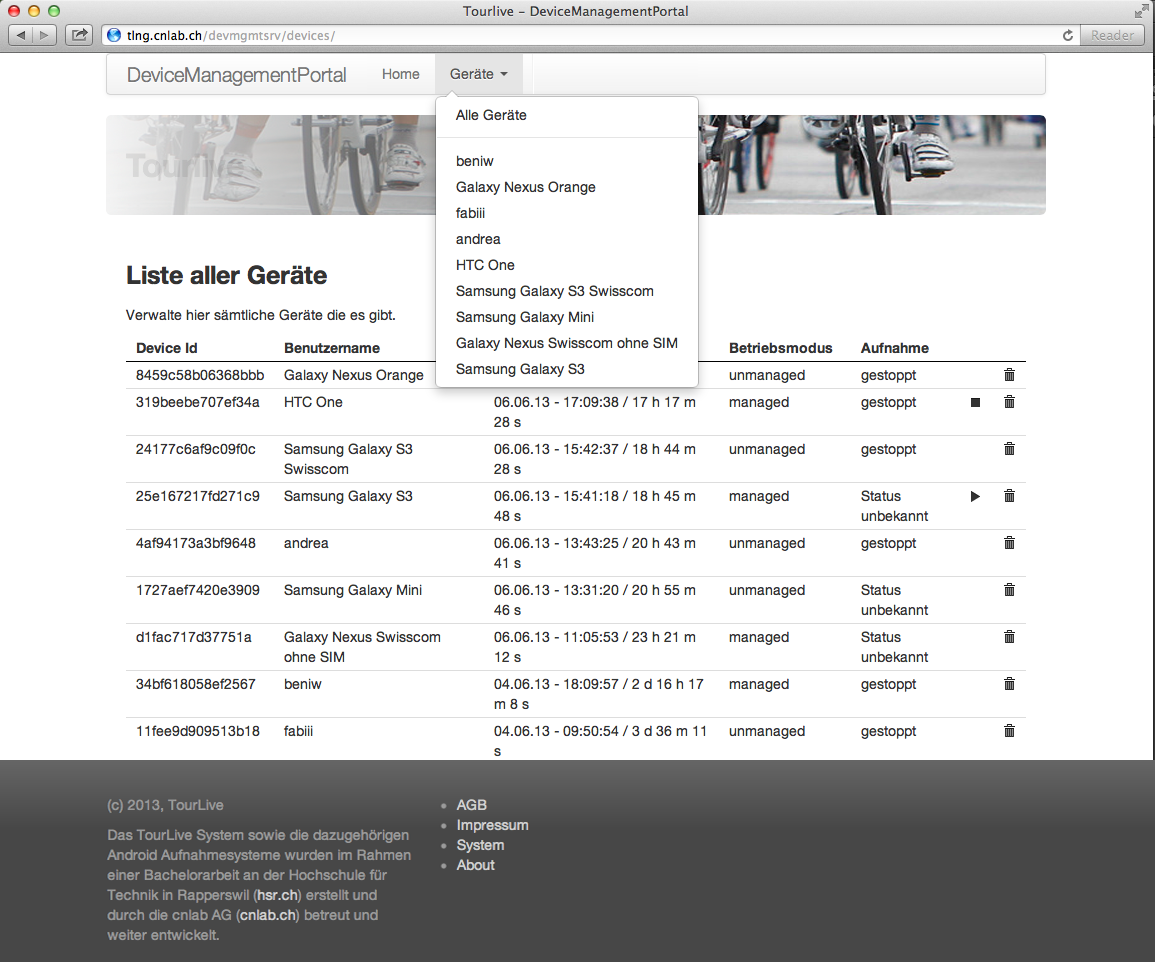
\includegraphics[width=120mm]{images/devmgmtsrv/all.png}
	\caption{Übersicht der Device Management Server Webseite}
\end{figure}

\subsubsection{Header}
Der Header bietet die Möglichkeit, über eine Schnellnavigation auf ein Gerät zuzugreifen. 
\begin{figure}[H]
	\centering
	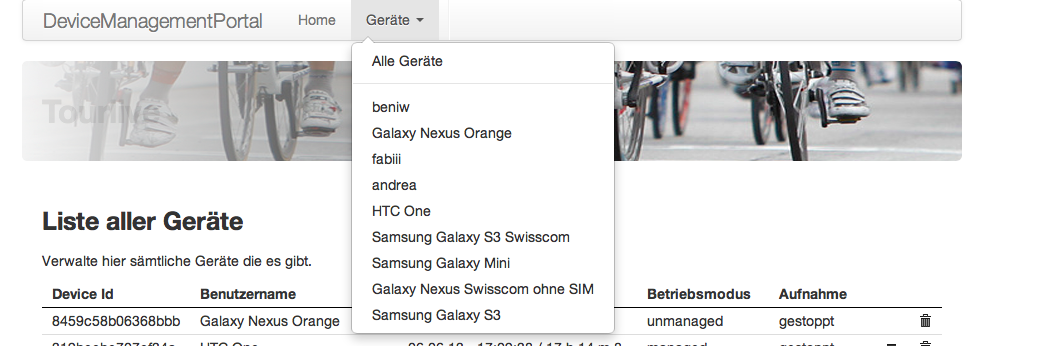
\includegraphics[width=120mm]{images/devmgmtsrv/header.png}
	\caption{Device Management Server Webseite - Header}
\end{figure}



\pagebreak
\subsubsection{Footer}
Der Footer enthält detaillierte Informationen zum Projekt TourLive. 
 
\begin{figure}[H]
	\centering
	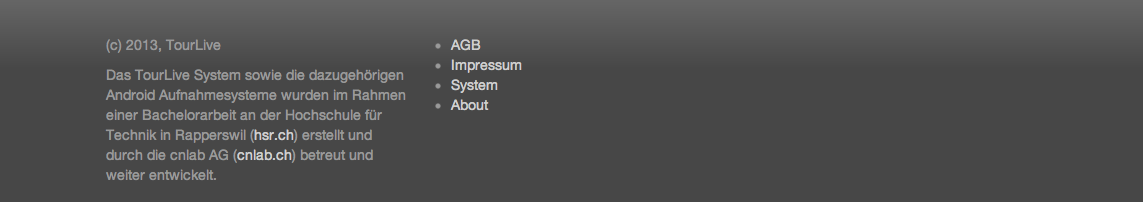
\includegraphics[width=120mm]{images/devmgmtsrv/footer.png}
	\caption{Device Management Server Webseite - Footer}
\end{figure}


\subsubsection{Hauptbereich}
Der Hauptbereich ist in zwei Teile unterteilt. So befindet sich Links eine Navigation, mit welcher zwischen den verschiedenen Funktionen navigiert werden kann. 
 
\begin{figure}[H]
	\centering
	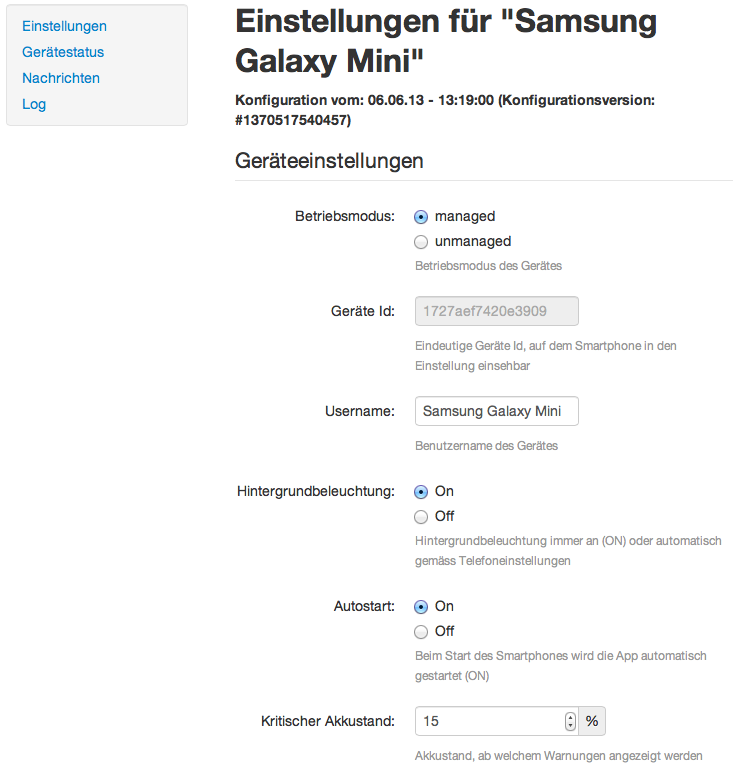
\includegraphics[width=120mm]{images/devmgmtsrv/settings.png}
	\caption{Device Management Server Webseite - Hauptbereich}
\end{figure}

